\documentclass{article}
\usepackage{graphicx}
\usepackage{siunitx}
\graphicspath{ {images/} }
\title{Ball Kick}
\author{Grant Curell}
\begin{document}
\maketitle{}
\section{Problem}
You’re at the tryouts for your favorite soccer team, with World Cup dreams on your mind. The only thing left is to prove that you can kick the ball far enough. The situation is as you see in Figure 4-12. You kick the ball at an angle $(\theta)$ with a certain speed, and you want to know how far the ball will go before hitting the ground. Say that $(\theta)$ = \ang{45} and that the initial speed of the ball is 50.0 meters/second. How far will it travel in the x direction before it hits the ground?
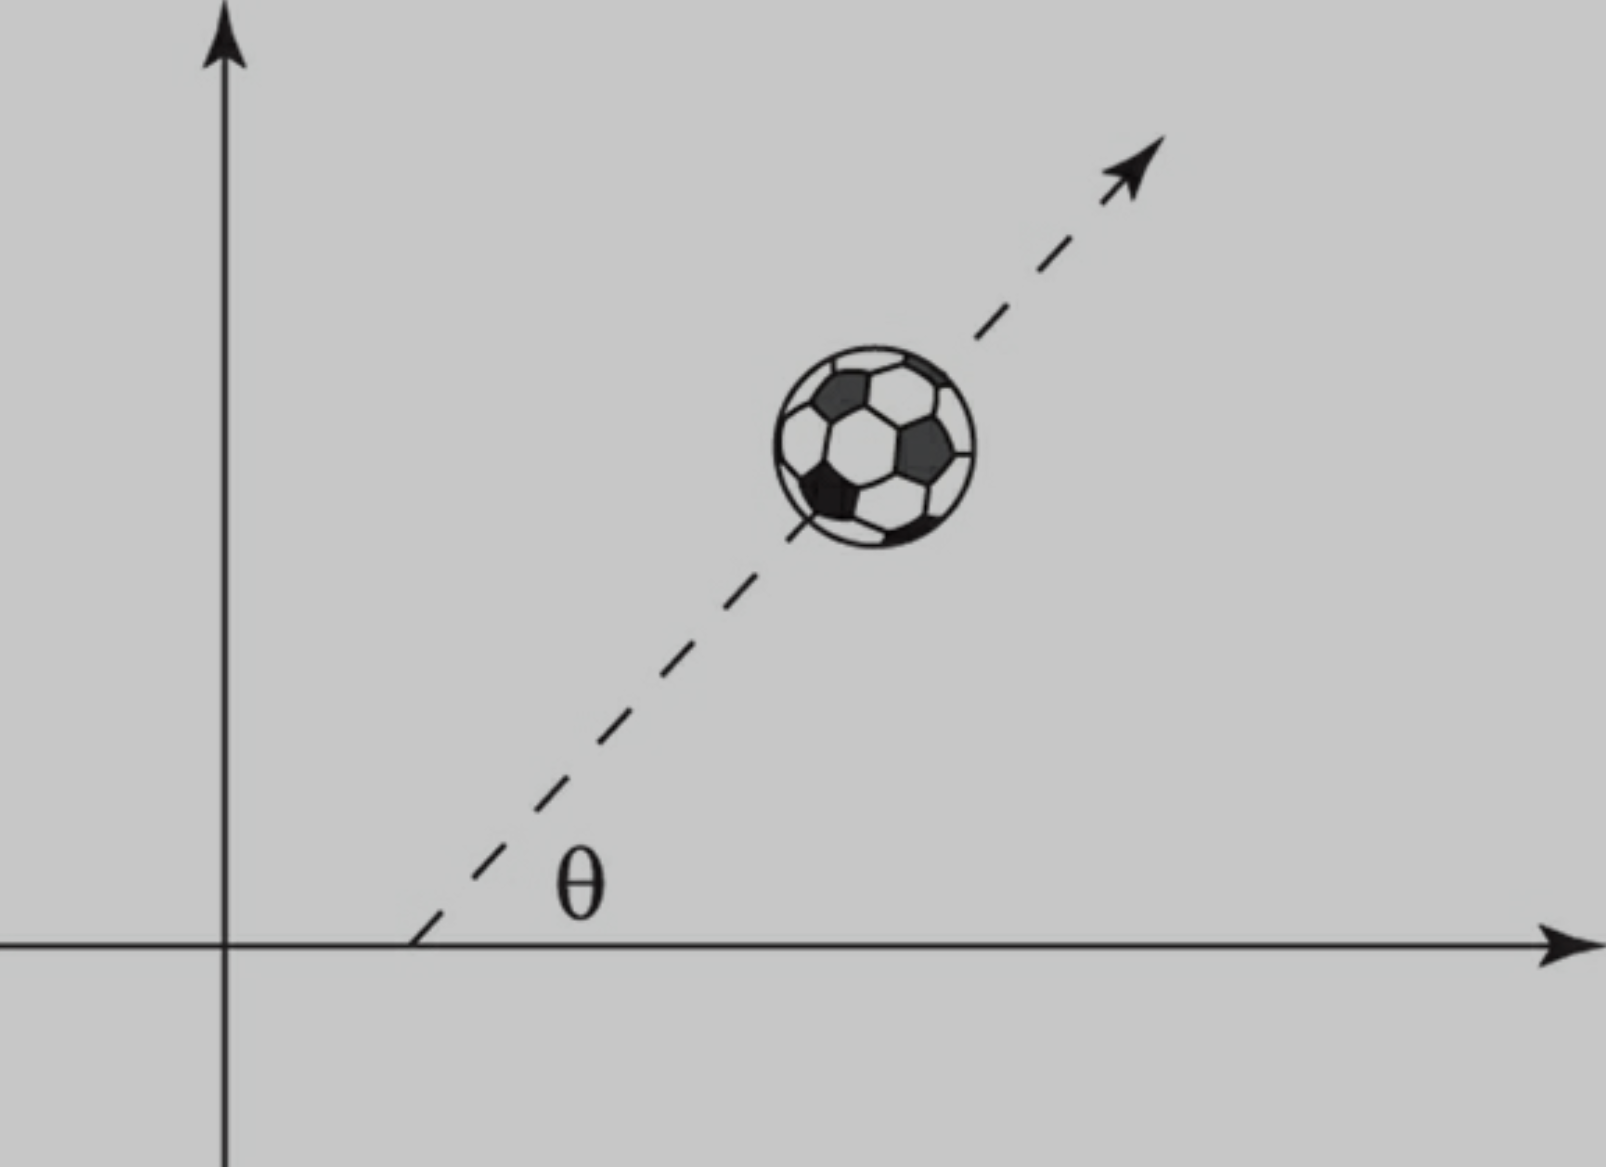
\includegraphics[width=\columnwidth]{image}
\\\\
Holzner, Steven. Physics I For Dummies (For Dummies (Math \& Science)) (p. 74). Wiley. Kindle Edition.
\\\\
\section{Solution}
\[ v_i=50m/s\ @\ \ang{45} \]
La primera pregunta es: cuanto tiempo hasta la pelota llegue al vértice de su trajectoria?
\[ v_f=0m/s \]
\[ a=\frac{\triangle{v}}{\triangle{t}} \]
\[ v_y=50\sin(45) \]
\[ -9.8 = \frac{-50\sin(45)}{t} \]
\[ t=\frac{-50\sin(45)}{-9.8} \]
\[ t=3.607 \]
Sería lo mismo para llegar al suelo así que:
\[ t=7.2s \]
\[ s=\bar{v}t \]
\[ s=50\cos(45)*7.2 \]
\[ s = 255m \]
La pelota rocorrería 255 metros antes de que llegue al suelo.
\end{document}
